\section{Обзор существующих методов}

Существует много алгоритмов для решения задачи семантической сегментации или задачи поиска контура. Сюда входят, в том числе, методы активного контура~\cite{snakes}, сегментация с помощью кластеризации~\cite{clustering_segm} и нейросетевые методы~\cite{fcn},~\cite{unet},~\cite{gridnet},~\cite{deeplab}.

\subsection{Простая сверточная модель}

\begin{table}[b]
  \begin{center}
    \caption{Структура сверточного блока} \label{tab:conv_block}
    \begin{tabular}{ c }
      \hline
      сверточный слой с~ядром~\kernel{3} + mvn     \\ \hline
      сверточный слой с~ядром~\kernel{3} + mvn     \\ \hline
      \dots                                        \\ \hline
      maxpool слой с~ядром~\kernel{2} и~шагом~2    \\ 
      \hline
    \end{tabular}
  \end{center}
\end{table}

\begin{figure}[ht]
  \includegraphics[width=\textwidth,keepratio]{img/fcn-1-layer-upsample}
  \caption{Схема архитектуры простой сверточной модели}
\end{figure}

Простая сверточная модель~\cite{fcn_1_layer_upsample} была разработана на основе сверточных нейронных сетей для классификации. Отличие состоит в том, что в сетях для класификации последний слой softmax~\cite{classification_loss} преобразует высокоуровневые признаки, полученные последовательным применением сверток в вероятности принадлежности к классам, а~для~сегментации сначала используется upsampling слой, который преобразует высокоуровневые признаки в~изображение размером с~исходное, которое описывает, где именно находится объект. Каждый сверточный блок состоит из~нескольких слоев, расположенных друг за~другом, как описано в~таблице~\ref{tab:conv_block}.

Такая структура часто используется в нейронных сетях, так~как~позволяет ускорить сходимость и~уменьшить количество вычислений при~сохранении точности. Сверточные слои обеспечивают вычисление высокоуровневых признаков с помощью применения фильтров к входному изображению. Maxpool слои позволяют уменьшить сложность вычислений, и оставить самую важную информацию, полученную из сверточных слоев. Слой dropout помогает избежать переобучения~\cite{dropout}. 

\subsection{FCN}

Модель с обратной сверткой~FCN~\cite{fcn} более сложная. Она состоит из~нескольких сверточных блоков и~нескольких обратных сверточных блоков. Каждый блок, в~свою очередь, состоит из~нескольких сверточных слоев с~функцией активации relu и~maxpool~слоя. 

\begin{figure}[ht]
  \includegraphics[width=\textwidth,keepratio]{img/fcn}
  \caption{Схема архитектуры FCN}
\end{figure}

Всего в~нейронной сети 3~сверточных блока и~1~блок без~maxpool слоя. Они идут подряд, и~каждый следующий на~выходе дает в~2~раза больше фильтров, чем~предыдущий. 
Структура обратного блока, напротив, нелинейная:

\begin{itemize}
  \item обратный сверточный слой с~ядром~\kernel{3} и~шагом~2,
  \item сверточный слой с~ядром~\kernel{1} и~шагом~1, который вычисляется от~предыдущего mvn~слоя~\cite{batch_norm},
  \item слой, который вычисляет среднее арифметическое из~первых двух слоев блока.
\end{itemize}

Всего в нейронной сети 3~обратных блока. 
Количество фильтров в каждой свертке обратного блока 
равно количеству классов. Если же класса всего~2, 
то мы задаем на выходе 1~фильтр и~в~конце используем 
функцию активации sigmoid, вычисляя ошибку при этом 
с~помощью индекса Дайса~\eqref{eq:dice_index}. 
В данной работе во~всех случаях используется только 2~класса.

Чтобы сеть сходилась устойчиво, после каждой свертки 
используется mvn слой. Преобразование входа~$X$ mvn~слоя 
описывается уравнением~\eqref{eq:mvn}. 

\begin{equation}
\label{eq:mvn_input_batch}
X\in{}R^{batch\_size\times{}n\times{}n\times{}filters}
\end{equation}

\begin{equation}
\label{eq:mvn_squared_batch}
(X^{2})_{i,j,k,t}=((X)_{i,j,k,t})^{2}
\end{equation}

\begin{equation}
\label{eq:mvn_expected_value}
E[X]=\frac{
  \sum_{i,j,k,t}X
}{
  n^{2}\times{}batch\_size\times{}filters
}
\end{equation} 

\begin{equation}
\label{eq:mvn}
Y(X)\ = \frac{
  X - E[X]
}{\sqrt{
  E[X^{2}] - (E[X])^2
}}
\end{equation}

Обратные сверточные слои 
позволяют получить карту вероятностей принадлежности 
входных пикселей объекту в~зависимости от~контекста 
из~высокоуровневых признаков, вычисленных сверточными слоями. 
Каждый блок обратной свертки связан не только с предыдущим блоком 
обратной свертки, но и с соответствующим по размеру сверточным блоком, 
для того, чтобы обеспечить сходимость сети. Несколько обратных слоев 
позволяют сгладить резкие переходы на~выходной карте вероятностей 
и~получить более точные предсказания. В~обратных блоках учитываются 
выходы соответствующих mvn слоев прямых блоков, чтобы увеличить 
скорость обучения. Этот~прием очень похож на~residual блоки в~\cite{resnet}.

\subsection{U-Net}

Архитектура U-Net~\cite{unet} основана на идеях, 
перечисленных при описании более простых моделей. 
Здесь также используются прямые и обратные блоки. 

\begin{figure}[hb]
  \includegraphics[width=\textwidth,keepratio]{img/unet}
  \caption{Схема архитектуры U-Net}
\end{figure}

Каждый прямой блок модели U-Net состоит из 2-х сверточных слоев 
с~ядром \kernel{3} и~функцией активации relu. В обратных блоках используются 
простые upsampling слои для получения изображения из высокоуровневых сетей. 
Кроме того, в обратных блоках присутствует concat слой, который конкатенирует 
выход соответствущего по размеру прямого блока и выход предыдущего обратного 
блока. Такое решение позволяет получать быструю сходимость сети, так как 
при~использовании алгоритма обратного распространения ошибки, последняя 
не~затухает, а сразу передается на~сверточные блоки. 

\subsection{GridNet}

\begin{figure}[ht]
  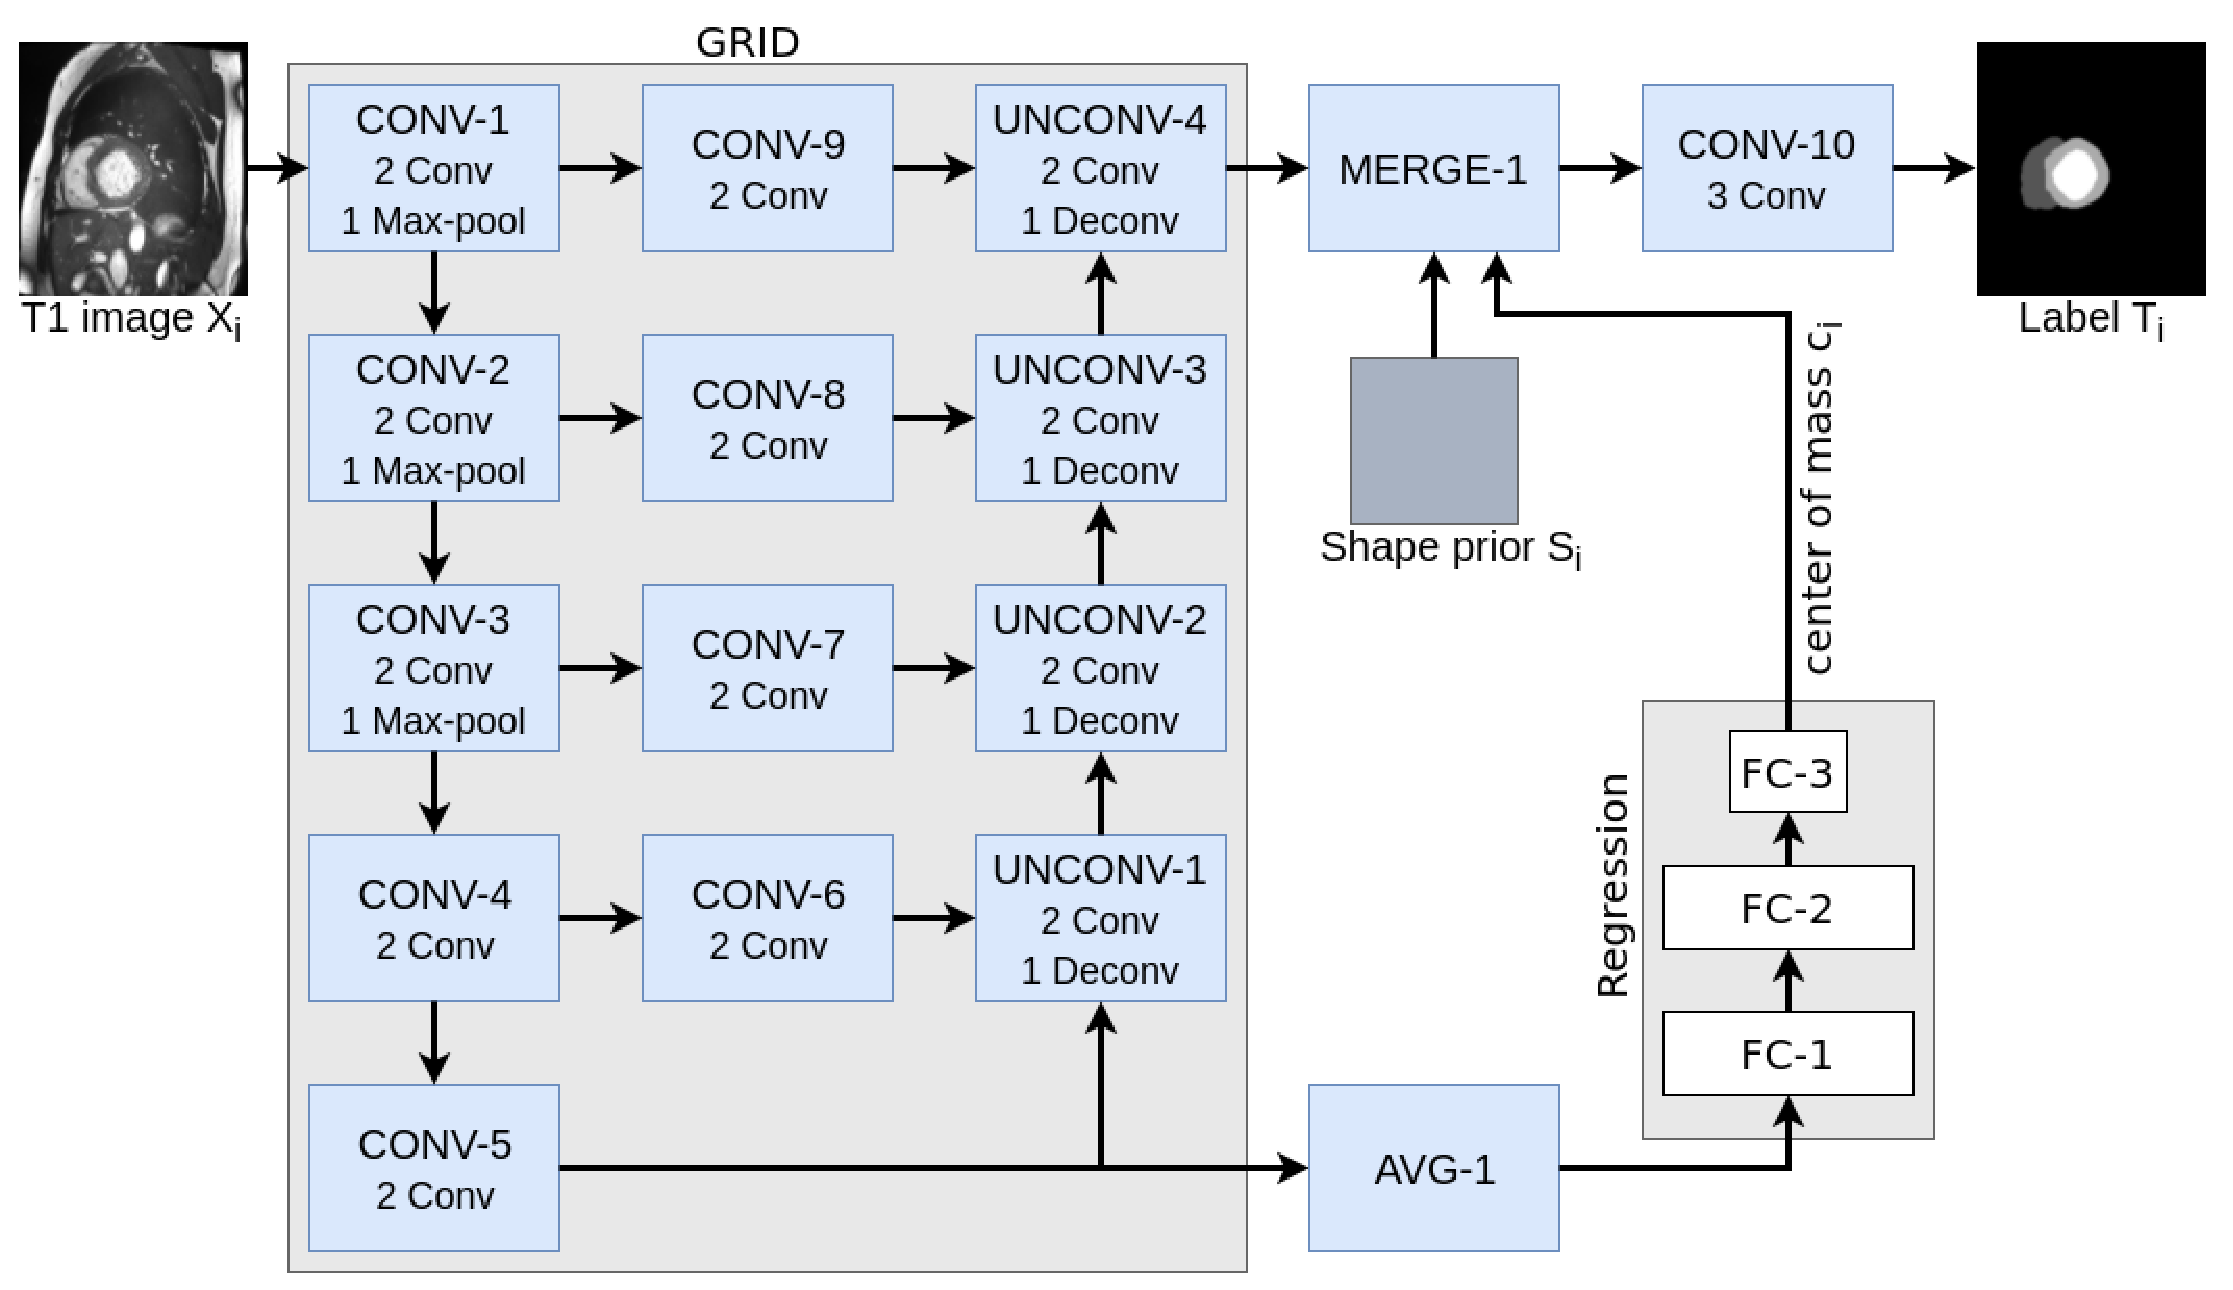
\includegraphics[width=\textwidth,keepratio]{img/gridnet}
  \caption{Схема архитектуры GridNet}
\end{figure}

Основная часть модели Gridnet~\cite{gridnet} заимствована у~U-Net. 
В~этой модели в~обратных блоках используется обратная свертка, 
а~также~добавляются дополнительные сверточные слои между~результатами 
свертки в~прямых блоках и~concat~слоем в~соответствующих обратных блоках. 
Эти измененения вместе~увеличивают количество параметров, но и~добавляют
точность сегментации.

\subsection{DenseNet}

\begin{figure}[ht]
  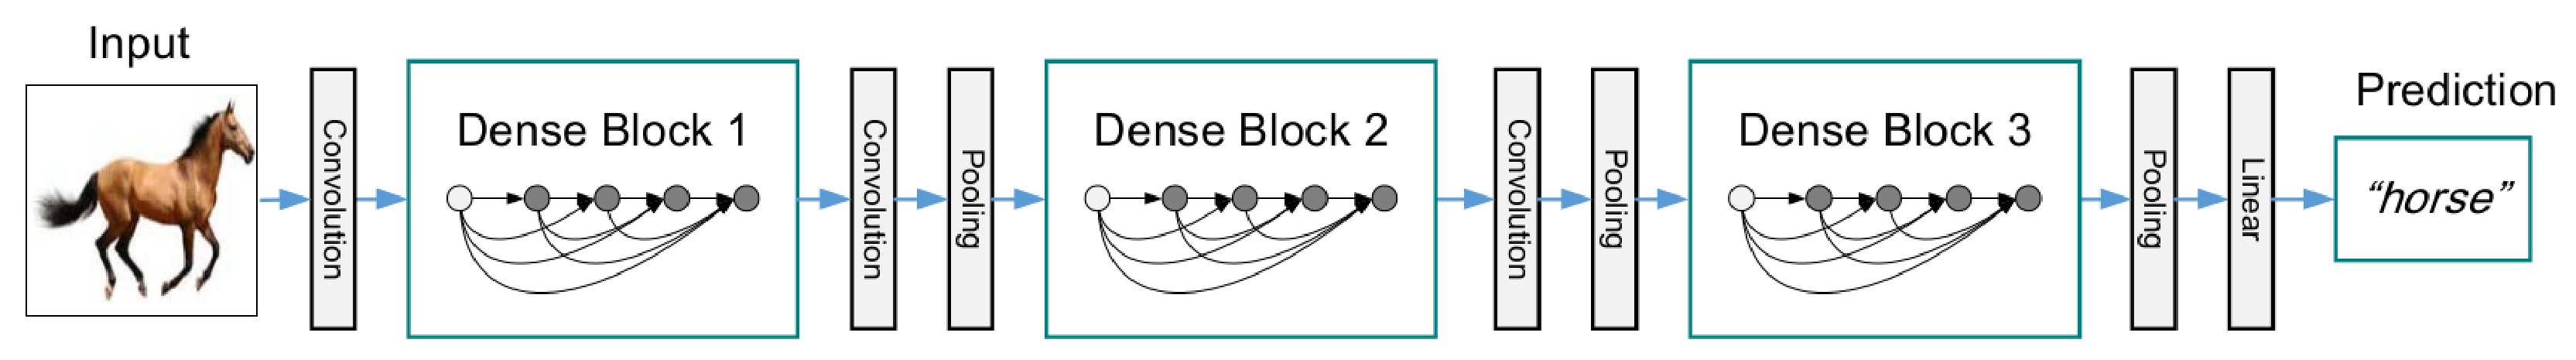
\includegraphics[width=\textwidth,keepratio]{img/densenet}
  \caption{Схема архитектуры DenseNet}
\end{figure}

Обычно между двумя maxpool слоями используется несколько подряд идущих сверточных слоев. Это позволяет сети преобразовывать более простые признаки в более сложные. Однако, в такой архитектуре возникают проблемы с алгоритмом обратного распространения ошибки, который используется для~обучения глубоких сетей. Возникает затухание градиента, поэтому обучение сети происходит только на последних слоях, а первые почти не изменяются. 

Новшество DenseNet~\cite{densenet} заключается в использовании dense сверточных блоков, которые являются альтернативой resnet блоков\cite{resnet}, предложенных для~решения описанной проблемы. Эти блоки располагаются между maxpool слоями, и каждый сверточный слой связан со всеми сверточными слоями этого блока, которые идут после него. Связь реализована с помощью concat слоя в~отличие от~resnet блоков, где используется просто сложение тензоров.   

\subsection{Растянутые сверточные слои}

Большинство сверточных сетей использует комбинацию сверточных слоев и~maxpool слоев. Из-за глубокой архитектуры это позволяет сверточным слоям учитывать большой контекст исходного изображения. Например, если сначала идет свертка 
с~ядром~\kernel{3}, а~затем maxpool с~ядром~\kernel{2}, то~следующая свертка 
с~ядром~\kernel{3} будет учитывать часть исходного изображения 
размером~\kernel{7}. С помощью использования большого контекста можно вовсе отказаться от полносвязных слоев в пользу сверточных, причем будет достаточно только слоев с ядром \kernel{3}.

Альтернативой слою maxpool являются растянутые сверточные 
слои~\cite{dilated_conv}. Идея заключается в~том, чтобы модифицировать ядро 
сверточного слоя так, что на входе пиксели матрицы будут учитываться 
через~один или~через~несколько. Такие слои используют меньше входов, 
но~охватывают большой контекст. 

\newpage

\begin{figure}[hb]
  \includegraphics[width=\textwidth,keepratio]{img/dilated-filter}
  \caption{Иллюстрация разрастания контекста при последовательном увеличении параметра растяжения слоев.}
\end{figure}

\DeclarePairedDelimiter\ceil{\lceil}{\rceil}
\DeclarePairedDelimiter\floor{\lfloor}{\rfloor}

Так, например, свертка с ядром \kernel{s},$s=3$ и растяжением $k=2$ 
\mbox{($m=\ceil{\frac{s+2(k-1)}{k}}=\ceil{\frac{5}{2}}=3$)} по~сути является 
сверткой~\kernel{5}, в которой используется только 9 входов~\eqref{eq:dilated_example}. 
Использование растянутых сверточных слоев показывает хорошие результаты~\cite{segm_dcnn_crf},~\cite{deeplab}.

\begin{equation}
\label{eq:dilated_example}
y = \sum_{
  \substack{
    i=0 \\
    j=0
  }
}^{m}x_{k\times{}i,k\times{}j}
\end{equation}

\iffalse
\subsection{DeepLab}
\fi

\subsection{Выводы}

Для решения задачи сегментации существует много конфигураций нейронных сетей, 
которые показывают хорошие результаты. Чтобы выбрать лучшую для~решения конкретной 
задачи сегментации снимков МРТ сердца, необходимо провести детальный анализ 
и~протестировать модели на одинаковых наборах данных. В таком случае можно 
объективно сравнивать результаты моделей.
